\documentclass{classes/exam} 
\usepackage{siunitx}
\usepackage{chemfig}
\usepackage{tikz}
\usepackage{physics}
\usepackage{circuitikz}
\usepackage{graphicx}
\graphicspath{ {./images/} }
\usepackage[version=4]{mhchem}
\usepackage{tkz-euclide}
\definecolor{myyellow}{RGB}{254,241,24}
\definecolor{myorange}{RGB}{234,125,1}
\definecolor{fancyorange1}{RGB}{253,138,9}
\definecolor{fancyorange2}{RGB}{246,156,123}
\definecolor{bittersweet}{rgb}{1.0, 0.44, 0.37}
\definecolor{brinkpink}{rgb}{0.98, 0.38, 0.5}
\definecolor{cadetgrey}{rgb}{0.57, 0.64, 0.69}
\definecolor{lightpink}{rgb}{1.0, 0.71, 0.76}
\usepackage{tkz-euclide}
\usetkzobj{all}
\tikzstyle arrowstyle=[scale=1]
\tikzstyle directed=[postaction={decorate,decoration={markings,
		mark=at position .65 with {\arrow[arrowstyle]{stealth}}}}]
\tikzstyle direct=[postaction={decorate,decoration={markings,
		mark=at position .65 with {\arrow[arrowstyle]{stealth reversed}}}}]
\usetikzlibrary{shadings,shapes.geometric,calc, patterns, angles, quotes, arrows.meta, shapes, decorations.pathmorphing, decorations.shapes, decorations.text,calc,angles,quotes,decorations.markings}
\tikzset{>=latex}
\usepackage{chemfig}
\usepackage{multirow}
\usetikzlibrary{quotes,arrows.meta}
%\pagestyle{empty}
\begin{document}
	\begin{center}
		{\kml ប្រឡងឆមាសលើកទី១ ថ្នាក់ទី១០\\
		វិញ្ញាសាៈ រូបវិទ្យា\\
		រយៈពេលៈ ៦០នាទី\\
		ពិន្ទុៈ ៥០}
	\end{center}
	\begin{enumerate}[I]
		\item {\color{magenta}\ks (១០ ពិន្ទុ)} ប្រអប់មួយមានទម្ងន់ $100\si{\newton}$ ស្ថិតនៅស្ងៀមនៅលើកម្រាលឥដ្ឋ។ ប្រសិនបើគេដឹងថា មេគុណកកិតស្តាទិចរវាងប្រអប់នេះ នឹងកម្រាលឥដ្ឋស្មើនឹង​ $0.4$។ គេឲ្យៈ $\cos30^\circ=0.86,~\sin30^\circ=0.50$\\
		ចូររកក​​ម្លាំងអប្បរមា $F$ ដែលត្រូវប្រើលើប្រអប់នេះដើម្បីឲ្យប្រអប់នេះចាប់ផ្តើមធ្វើចលនា(ដូចរូប)។
		\begin{figure}[H]
			\centering
			\begin{tikzpicture}[>=Stealth]
				\coordinate (O) at (0,.1);
				\coordinate (A) at (3.5,.5);
				\coordinate (B) at (5,.5);
				\coordinate (F) at (5,1.5);
				\fill[pattern=bricks, pattern color=black, preaction={fill=lightpink}] (O) rectangle (6,-.3);
				\filldraw[gray!40!black,fill=cadetgrey] (2.5,.1) rectangle (3.5,1);
				\draw[->, line width=2pt] (A)--(F);
				\draw[dashed] (A)--(B);
				\node[right] at (5,1.4) {$\overrightarrow{F}$};
				\pic [draw, ->, "$30^\circ$", angle eccentricity=1.5, angle radius=1cm] {angle = B--A--F};
			\end{tikzpicture}
		\end{figure}
		\item {\color{magenta}\ks (១០ ពិន្ទុ)} នៅចុងខ្សែមួយបានចងភ្ជាប់នឹងកូនជញ្ជីង $50\si{\kilogram}$។ គេទាញកូនជញ្ជីងចេញពីទីតាំងលំនឹងបានមុំ $30^\circ$។\\ រកកម្លាំងដែលទាញកូនជញ្ជីងពីទីតាំងលំនឹង និងតំណឹងនៃខ្សែ។ គេឲ្យៈ $\cos30^\circ=0.86,~\sin30^\circ=0.50$
		\begin{figure}[H]
			\centering
			\begin{tikzpicture}[>=stealth]
				\begin{scope}
					\coordinate (centre) at (0,0);
					\coordinate (force) at (3.5,-2.3);
					\draw[dashed,gray] (centre) -- ++ (0,-1) node (mary) [black,below]{$ $};
					\draw[magenta] (centre) -- ++(310:3) coordinate (block);
					\draw[->] (block)--(force) node[above] (force) {$\overrightarrow{F}$};
					\draw[<-, magenta, >=Latex] (310:1.5) -- (block);
					\draw[->, magenta, >=Latex] (1.9,-2.5) -- (1.9,-3.5) node[below] (1.9,-3.5) {$\overrightarrow{w}=m\vec{g}$};
					\node[circle,outer color=teal,inner color=white,minimum width=.8cm] (radial) at (block) {};
					\pic [draw, ->, "$30^\circ$", angle eccentricity=1.5, angle radius=1cm] {angle = mary--centre--block};
					\draw [line width=2pt] (-.6,0) -- (.6,0);
					\fill[bottom color=gray, top color=gray!40!white] ($ (centre) + (-.6,0) $) rectangle ($ (centre) + (.6,0.2) $);
					\coordinate (m) at (block);
					\node at (1.3,-1) {$\overrightarrow{T}$};
				\end{scope}
			\end{tikzpicture}
		\end{figure}
		\item {\color{magenta}\ks (១៥ ពិន្ទុ)} ចលនាត្រង់មួយមានសមីការ $x=10+20t-5t^{2}$ ដោយ $x$ គិតជាម៉ែត្រ $\left(\si{\metre}\right)$ និង $t$ គិតជាវិនាទី $\left(\si{\second}\right)$ ។
		\begin{enumerate}[k]
			\item កំណត់ប្រភេទនៃចលនា និងគណនាសំទុះ។
			\item គណនាល្បឿនខណៈនៅខណៈពេល $t=0$ និង $t=2\si{\second}$។
			\item តើចល័តស្ថិតនៅទីតាំងណា នៅខណៈដែលល្បឿនរបស់វាមានតម្លៃស្មើសូន្យ។
		\end{enumerate}
		\item {\color{magenta}\ks (១៥ ពិន្ទុ)} ពិនិត្យមើលរូបខាងក្រោម។ អង្គធាតុ $A$ មានម៉ាស $5.0\si{\kilogram}$ អង្គធាតុ $B$ មានម៉ាស $2.0\si{\kilogram}$ ត្រូវបានចងភ្ជាប់គ្នាដោយខ្សែមិនយឺត មិននិងមិនគិតម៉ាសហើយឆ្លងកាត់រ៉កមួយ។ គេឃើញអង្គធាតុ $A$ ផ្លាស់ទីទៅស្តាំឯអង្គធាតុ $B$ ផ្លាស់ទីទៅខាងឆ្វេង។
		ចូរកំណត់សំទុះ និងតំណឹងខ្សែនៃប្រព័ន្ធ។ មេគុណកកិតរវាងអង្គធាតុ $A$ នឹងផ្ទៃតុគឺ $0.2$។
		\begin{figure}[H]
			\centering
			\begin{tikzpicture}
			\coordinate (O) at (0,0);
			\node at (O) {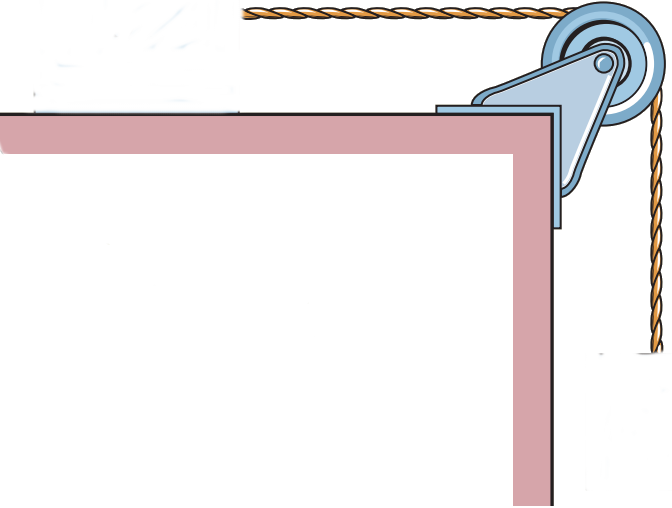
\includegraphics[scale=.22]{pulley_system}};
			\draw[fill=white] (2.5,0) circle (.15cm);
			\draw[fill=white] (0,1.87) circle (.15cm);
			\filldraw[gray!40!black,fill=cadetgrey] (-1.5,1.1) rectangle (0,2.8);
			\filldraw[gray!40!black,fill=cadetgrey] (2,0) rectangle (3,-1);
			\node at (-.7,2) {$A$};
			\node at (2.46,-.5) {$B$};
			\end{tikzpicture}
		\end{figure}
	\end{enumerate}
\newpage
\begin{center}
	{\kml ប្រឡងឆមាសលើកទី១ ថ្នាក់ទី១០\\
		វិញ្ញាសាៈ រូបវិទ្យា\\
		រយៈពេលៈ ៦០នាទី\\
		ពិន្ទុៈ ៥០}
\end{center}
{\kml អត្រាកំណែ}
\begin{enumerate}[I]
	\item {\color{magenta}\ks (១០ ពិន្ទុ)} ចូររកក​​ម្លាំងអប្បរមា $F$ ដែលត្រូវប្រើលើប្រអប់នេះដើម្បីឲ្យប្រអប់នេះចាប់ផ្តើមធ្វើចលនា
	\begin{figure}[H]
		\centering
		\begin{tikzpicture}[>=Stealth]
				\coordinate (O) at (0,.1);
				\coordinate (A) at (3.5,.5);
				\coordinate (B) at (5.5,.5);
				\coordinate (F) at (5.5,2);
				\filldraw[gray!40!black,fill=cadetgrey] (2.5,0) rectangle (3.5,1);
				\draw[->, line width=2pt] (A)--(F);
				\draw[->] (A)--(B) node[right] (B) {$\overrightarrow{F}_{x}$};
				\node[right] at (5.5,2) {$\overrightarrow{F}$};
				\pic [draw, ->, "$30^\circ$", angle eccentricity=1.5, angle radius=1cm] {angle = B--A--F};
				\draw[->] (3,.5) to (3,-1) node[below] (3,-1) {$\overrightarrow{w}$};
				\draw[->] (3,0) to (1.5,0) node[left] (1.5,0) {$\overrightarrow{f}_{s}$};
				\draw[->] (3,0) to (3,2) node[above] (3,2) {$\overrightarrow{F}_{N}$};
				\draw[->] (3.5,.5) to (3.5,2) node[above] (3.5,2) {$\overrightarrow{F}_{y}$};
				\draw[dashed] (F) to (5.5,.5);
				\draw[dashed] (F) to (3.5,2);
		\end{tikzpicture}
	\end{figure}
	\begin{align*}
		\text{លក្ខខណ្ឌលំនឹង}\quad :&\quad \Sigma \overrightarrow{F}=\vec{0}~\text{ឬ}~\overrightarrow{F}+\overrightarrow{f}_{s}+\overrightarrow{F}_{N}+\overrightarrow{w}=\vec{0}\\
		\text{តាម $\left(ox\right)$}\quad :&\quad \overrightarrow{F}_{x}+\overrightarrow{f}_{s}=\vec{0}~\text{នោះ}~F_{x}-f_{s}=0\\
		\quad :&\quad F_{x}=f_{s}~\text{ឬ}~F\cos30^\circ=f_{s}\\
		\text{តែ}\quad :&\quad f_{s}=\mu_{s}F_{N}\\
		\text{គេបាន}\quad :&\quad F\cos30^\circ=\mu_{s}F_{N}\quad(1)\\
		\text{តាម$\left(oy\right)$}\quad :&\quad \overrightarrow{F}_{N}+\overrightarrow{w}+\overrightarrow{F}_{y}=\vec{0}~\text{នោះ}~F_{N}-w+F_{y}=0\\
		\text{ម្យ៉ាងទៀត}\quad :&\quad F_{N}=w-F\sin30^\circ\quad(2)\\
		\text{យកសមីការ $(2)$ ជំនួសក្នុងសមីការ $(1)$}\\
		\text{គេបាន}\quad :&\quad F\cos30^\circ = \mu_{s}\left(w-F\sin30^\circ\right)\\
		\quad :&\quad F\cos30^\circ = \mu_{s}w-\mu_{s}F\sin30^\circ\\
		\text{នាំឲ្យ}\quad :& \quad F=\frac{\mu_{s}w}{\cos30^\circ+\mu_{s}\sin30^\circ}\\
		\text{ដោយ}\quad :&\quad \mu_{s}=0.4,~w=100N,~\cos30^\circ=0.86,~\sin30=0.50\\
		\text{គេបាន}\quad :&\quad F=\frac{0.4\times100}{0.86+0.4\times 0.5}=37.7N\\
		\text{ដូចនេះ}\quad :&\quad F=37.7N
	\end{align*}
	\item {\color{magenta}\ks (១០ ពិន្ទុ)} រកកម្លាំងដែលទាញកូនជញ្ជីងពីទីតាំងលំនឹង និងតំណឹងនៃខ្សែ
	\begin{figure}[H]
		\centering
		\begin{tikzpicture}[>=stealth]
		\begin{scope}
			\coordinate (centre) at (0,0);
			\coordinate (force) at (3.5,-2.3);
			\coordinate (R) at (3.5,-4);
			\coordinate (w) at (1.9,-4);
			\draw[dashed,gray] (centre) -- ++ (0,-1) node (mary) [black,below]{$ $};
			\draw[magenta] (centre) -- ++(310:3) coordinate (block);
			\draw[->] (block)--(force) node[above] (force) {$\overrightarrow{F}$};
			\draw[<-, magenta, >=Latex] (310:1) -- (block);
			\draw[->, magenta, >=Latex] (1.9,-2.5) -- (w) node[below] (w) {$\overrightarrow{w}=m\vec{g}$};
			\draw[->] (block) to (R);
			\node[circle,outer color=teal,inner color=white,minimum width=.8cm] (radial) at (block) {};
			\pic [draw, ->, "$30^\circ$", angle eccentricity=1.5, angle radius=1cm] {angle = mary--centre--block};
			\draw [line width=2pt] (-.6,0) -- (.6,0);
			\fill[bottom color=gray, top color=gray!40!white] ($ (centre) + (-.6,0) $) rectangle ($ (centre) + (.6,0.2) $);
			\coordinate (m) at (block);
			\node at (1.3,-1) {$\overrightarrow{T}$};
			\draw[dashed] (1.9,-4) to (R);
			\node[right] at (R) {$\vec{R}$};
			\draw[dashed] (R) to (force);
			\pic [draw, ->, "$30^\circ$", angle eccentricity=1.5, angle radius=1cm] {angle = w--block--R};
		\end{scope}
		\end{tikzpicture}
		\begin{align*}
			\text{លក្ខខណ្ឌលំនឹង}\quad :&\quad \Sigma \overrightarrow{F}=\vec{0}~\text{នោះ}~\overrightarrow{T}+\overrightarrow{R}+\overrightarrow{F}+\overrightarrow{w}=\vec{0}\\
			\text{ដោយ}\quad :&\quad \overrightarrow{T} + \overrightarrow{R}=\vec{0}~\text{នោះ}~T-R=0,~\text{ឬ}~T=R\\
			\text{ម្យ៉ាងទៀត}\quad :&\quad w=R\cos 30^\circ~\text{និង}~F=R\sin 30^\circ\\
			\text{ផលធៀប}\quad :&\quad \frac{F}{w}=\frac{R\sin 30^\circ}{R\cos 30^\circ}\\
			\text{នាំឲ្យ}\quad :&\quad F=\frac{w\sin 30^\circ}{\cos 30^\circ}=\frac{mg\sin 30^\circ}{\cos 30^\circ}\\
			\text{ដោយ}\quad :&\quad m=50\si{\kilogram},~g=9.80\si{\metre/\second^{2}}\\
			\text{គេបាន}\quad :&\quad F=\frac{50\times 9.80\times 0.5}{0.86}=284.88\si{\newton}\\
			\text{និង}\quad :& \quad T=R=\frac{W}{\cos 30^\circ}=\frac{mg}{\cos 30^\circ}\\
			\text{គេបាន}\quad :&\quad T=\frac{50\times 9.80}{0.86}=569.76\si{\newton}\\
			\text{ដូចនេះ}\quad :&\quad F=284.88\si{\newton}~\text{និង}~ T=569.76\si{\newton}\\
		\end{align*}
	\end{figure}
	\item {\color{magenta}\ks (១៥ ពិន្ទុ)}
	\begin{enumerate}[k]
		\item កំណត់ប្រភេទនៃចលនា និងគណនាសំទុះ។
		\begin{align*}
			\text{យើងមាន}\quad :&\quad x=10+20t-5t^{2}\\
			\text{មានរាង}\quad :&\quad x=x_{0}+v_{o}t+\frac{1}{2}at^{2}\\
			\text{យើងបាន}\quad :&\quad \frac{1}{2}a=-5~\Rightarrow a=-10\si{\metre/\second^{2}},~v_{0}=20\si{\metre/\second},~x_{0}=10\si{\metre}\\
			\text{ដូចនេះ}\quad :&\quad a=-10\si{\metre/\second^{2}}<0~\text{ប្រភេទចលនារបស់ចល័តជាចលនាយឺតស្មើ។}
		\end{align*}
		\item គណនាល្បឿនខណៈនៅខណៈពេល $t=0$ និង $t=2\si{\second}$។
			\begin{align*}
				\text{តាមរូបមន្ត}\quad :&\quad v=v_{0}+at\\
				\text{បើ}\quad :&\quad t=0\si{\second},~a=-10\si{\metre/\second^{2}},~v_{0}=20\si{\metre/\second}\\
				\text{គេបាន}\quad :&\quad v=20-10\left(0\right)=20\si{\metre/\second}\\
				\text{បើ}\quad :&\quad t=2\si{\second},~a=-10\si{\metre/\second^{2}},~v_{0}=20\si{\metre/\second}\\
				\text{គេបាន}\quad :&\quad v=20-10\left(2\right)=0\si{\metre/\second}
			\end{align*}
		\item តើចល័តស្ថិតនៅទីតាំងណា នៅខណៈដែលល្បឿនរបស់វាមានតម្លៃស្មើសូន្យ។
		\begin{align*}
			\text{យើងមាន}\quad :&\quad x=\left(10+20t-5t^{2}\right)m~\text{ហើយល្បឿនស្មើសូន្យកាលណា}~t=2\si{\second}\\
			\text{គេបាន}\quad :&\quad x=10+20\left(2\right)-5\left(2\right)^{2}=30\si{\metre}\\
			\text{ដូចនេះ}\quad :&\quad\text{នៅខណៈ}~t=2\si{\second},~ x=30\si{\metre}
		\end{align*}
	\end{enumerate}
	\item {\color{magenta}\ks (១៥ ពិន្ទុ)} ចូរកំណត់សំទុះ និងតំណឹងខ្សែនៃប្រព័ន្ធ
	\begin{figure}[H]
		\centering
		\begin{tikzpicture}
			\coordinate (O) at (0,0);
			\draw[->] (0,1) to (-3,1) node[left] (-3,1) {$\overrightarrow{f}_{k}$};
			\draw[->] (-.7,2) to (1.5,2) node[right] (1.5,2) {$\overrightarrow{T}$};
			\draw[->] (-.7,1.5) to (-.7,4) node[above] (-.7,4) {$\overrightarrow{F}_{N}$};
			\draw[->] (-.7,1.5) to (-.7,-.5) node[below] (-.7,-.5) {$\overrightarrow{w}_{A}$};
			\filldraw[gray!40!black,fill=cadetgrey] (-1.5,1) rectangle (0,2.8);
			\draw[->] (4.46,1.5) to (4.46,3) node[above] (4.46,3) {$\overrightarrow{T}$};
			\draw[->] (4.46,1.5) to (4.46,0) node[below] (4.46,0) {$\overrightarrow{w}_{B}$};
			\filldraw[gray!40!black,fill=cadetgrey] (4,1) rectangle (5,2);
			\node at (-.7,2) {$A$};
			\node at (4.46,1.5) {$B$};
		\end{tikzpicture}
	\end{figure}
	\begin{itemize}
		\item ចំពោះអង្គធាតុ $A$
			\begin{align*}
				\text{គោលការណ៍គ្រឹះនៃឌីណាមិច}\quad :&\quad \Sigma \vec{F}=m_{A}\vec{a}\\
				\text{គេសរសេរ}\quad :&\quad \overrightarrow{f}_{k}+\overrightarrow{T}+\overrightarrow{w}_{A}+\overrightarrow{F}_{N}=m_{A}\vec{a}\quad
				\text{តែ}\quad \overrightarrow{w}_{A}+\overrightarrow{F}_{N}=\vec{0}\\
				\text{ជាតម្លៃ}\quad :&\quad T-f_{k}=m_{A}a~\text{ឬ}~T=m_{A}a+f_{k}\quad
				\text{ដែល}\quad f_{k}=\mu_{k}m_{A}g\\
				\text{គេបាន}\quad :&\quad T=m_{A}a+\mu_{k}m_{A}g\quad (1)
			\end{align*}
		\item ចំពោះអង្គធាតុ $B$
			\begin{align*}
				\text{គោលការណ៍គ្រឹះនៃឌីណាមិច}\quad :&\quad \Sigma \vec{F}=m_{B}\vec{a}\\
				\text{គេសរសេរ}\quad :&\quad \overrightarrow{w}_{B}+\overrightarrow{T}=m_{B}\vec{a}\\
				\text{ជាតម្លៃ}\quad :&\quad W_{B}-T=m_{B}a~\text{ឬ}~m_{B}g-T=m_{B}a\\
				\text{គេបាន}\quad :&\quad T=m_{B}g-m_{B}a\quad (2)\\
				\text{តាមសមីការ $\left(1\right)$ និង $\left(2\right)$}\\
				\text{គេបាន}\quad :&\quad m_{A}a+\mu_{k}m_{A}g=m_{B}g-m_{B}a\\
				\text{នាំឲ្យ}\quad :&\quad a=\frac{\left(m_{B}-\mu_{k}m_{A}\right)g}{m_{A}+m_{B}},\quad m_{A}=5\si{\kilogram},~m_{B}=2\si{\kilogram},~\mu_{k}=0.2,~g=9.80\si{\metre/\second^{2}}\\
				\text{គេបាន}\quad :&\quad a=\frac{\left(2-0.2\cdot 5\right)9.80}{5+2}=1.4\si{\metre/\second^{2}}\\
				\text{តាមសមីការ $\left(2\right)$}\quad :&\quad T=m_{B}g-m_{B}a=\left(g-a\right)m_{B}=\left(9.80-1.4\right)2=16.8\si{\newton}\approx 17\si{\newton}\\
				\text{ដូចនេះ}\quad :&\quad a=1.4\si{\metre/\second^{2}}~\text{និង}~T=17\si{\newton}
			\end{align*}
	\end{itemize}
\end{enumerate}
\end{document}